\documentclass[]{article}
\usepackage{lmodern}
\usepackage{amssymb,amsmath}
\usepackage{ifxetex,ifluatex}
\usepackage{fixltx2e} % provides \textsubscript
\ifnum 0\ifxetex 1\fi\ifluatex 1\fi=0 % if pdftex
  \usepackage[T1]{fontenc}
  \usepackage[utf8]{inputenc}
\else % if luatex or xelatex
  \ifxetex
    \usepackage{mathspec}
    \usepackage{xltxtra,xunicode}
  \else
    \usepackage{fontspec}
  \fi
  \defaultfontfeatures{Mapping=tex-text,Scale=MatchLowercase}
  \newcommand{\euro}{€}
\fi
% use upquote if available, for straight quotes in verbatim environments
\IfFileExists{upquote.sty}{\usepackage{upquote}}{}
% use microtype if available
\IfFileExists{microtype.sty}{%
\usepackage{microtype}
\UseMicrotypeSet[protrusion]{basicmath} % disable protrusion for tt fonts
}{}
\ifxetex
  \usepackage[setpagesize=false, % page size defined by xetex
              unicode=false, % unicode breaks when used with xetex
              xetex]{hyperref}
\else
  \usepackage[unicode=true]{hyperref}
\fi
\usepackage[usenames,dvipsnames]{color}
\hypersetup{breaklinks=true,
            bookmarks=true,
            pdfauthor={Ivo Hofacker, Dominik Steininger, Sven Findeiß, and many more\\},
            pdftitle={ViennaRNA Tutorial},
            colorlinks=true,
            citecolor=blue,
            urlcolor=blue,
            linkcolor=magenta,
            pdfborder={0 0 0}}
\urlstyle{same}  % don't use monospace font for urls
\usepackage{longtable,booktabs}
\usepackage{graphicx,grffile}
\makeatletter
\def\maxwidth{\ifdim\Gin@nat@width>\linewidth\linewidth\else\Gin@nat@width\fi}
\def\maxheight{\ifdim\Gin@nat@height>\textheight\textheight\else\Gin@nat@height\fi}
\makeatother
% Scale images if necessary, so that they will not overflow the page
% margins by default, and it is still possible to overwrite the defaults
% using explicit options in \includegraphics[width, height, ...]{}
\setkeys{Gin}{width=\maxwidth,height=\maxheight,keepaspectratio}
\setlength{\parindent}{0pt}
\setlength{\parskip}{6pt plus 2pt minus 1pt}
\setlength{\emergencystretch}{3em}  % prevent overfull lines
\providecommand{\tightlist}{%
  \setlength{\itemsep}{0pt}\setlength{\parskip}{0pt}}
\setcounter{secnumdepth}{0}

\title{ViennaRNA Tutorial}
\date{2017-08-02 20:50:00}
\author{Ivo Hofacker, Dominik Steininger, Sven Findeiß, and many more}
% Redefines (sub)paragraphs to behave more like sections
\ifx\paragraph\undefined\else
\let\oldparagraph\paragraph
\renewcommand{\paragraph}[1]{\oldparagraph{#1}\mbox{}}
\fi
\ifx\subparagraph\undefined\else
\let\oldsubparagraph\subparagraph
\renewcommand{\subparagraph}[1]{\oldsubparagraph{#1}\mbox{}}
\fi
\newcommand\todo[1]{\color{red}#1\color{black}}

\begin{document}
\maketitle


\includegraphics{Figs/unilogo_small.png}

\href{http://www.tbi.univie.ac.at/}{Theoretical Biochemistry Group}
\href{https://www.tbi.univie.ac.at/index.html}{
\includegraphics{Figs/tbilogo.png}}

\href{https://www.tbi.univie.ac.at/software}{Software}
\href{https://www.tbi.univie.ac.at/RNA/index.html}{ViennaRNA}
\href{https://www.tbi.univie.ac.at/RNA/tutorial/tutorial.html}{Tutorial}

\section{A short Tutorial on RNA Bioinformatics\\
The ViennaRNA Package and related Programs}
\url{http://www.tbi.univie.ac.at/RNA/}\\

This tutorial aims to give a basic introduction to using the programs
in the ViennaRNA Package.

\subsection{Get started}\label{get-started}

\subsubsection{What's in the \texttt{ViennaRNA\ Package}}{What's in the ViennaRNA Package}\label{whats-in-the-viennarna-package}

The core of the \texttt{ViennaRNA\ Package} is formed by a collection
of routines for the prediction and comparison of RNA secondary
structures.  These routines can be accessed through stand-alone
programs, such as \texttt{RNAfold}, \texttt{RNAdistance} etc., which
should be sufficient for most users. For those who wish to develop
their own programs a library which can be linked to your own code is
provided.

\paragraph{Which programs are available?}\\
\begin{itemize}
\item \texttt{RNA2Dfold} Compute coarse grained energy landscape of representative
sample structures \\
\item \texttt{RNAaliduplex} Predict conserved RNA-RNA interactions
between two alignments\\
\item {\bf TODAY} \texttt{RNAalifold} Calculate secondary structures for a set of aligned RNA sequences\\
\item {\bf TODAY} \texttt{RNAcofold} Calculate secondary structures of two RNAs with dimerization\\
\item \texttt{RNAdistance} Calculate distances between RNA secondary structures \\
\item {\bf TODAY} \texttt{RNAduplex} Compute the structure upon hybridization of two RNA strands\\
\item \texttt{RNAeval} Evaluate free energy of RNA sequences with given secondary structure\\
\item {\bf TODAY} \texttt{RNAfold} Calculate minimum free energy secondary structures and partition function of RNAs\\
\item \texttt{RNAheat} Calculate the specific heat (melting curve) of an RNA sequence
\item \texttt{RNAinverse} Find RNA sequences with given secondary structure (sequence design)
\item \texttt{RNALalifold} Calculate locally stable secondary structures for a set of aligned RNAs\\
\item \texttt{RNALfold} Calculate locally stable secondary structures of long RNAs\\
\item \texttt{RNApaln} RNA alignment based on sequence base pairing propensities\\
\item \texttt{RNApdist} Calculate distances between thermodynamic RNA secondary structures ensembles\\
\item \texttt{RNAparconv} Convert energy parameter files from ViennaRNA 1.8 to 2 format\\
\item \texttt{RNAPKplex} Predict RNA secondary structures including pseudoknots\\
\item \texttt{RNAplex} Find targets of a query RNA\\
\item \texttt{RNAplfold} Calculate average pair probabilities for locally stable secondary structures\\
\item \texttt{RNAplot} Draw and markup RNA secondary structures in PostScript, SVG, or GML\\
\item \texttt{RNApvmin} Find a vector of perturbation energies which may further be used to constrain folding\\
\item \texttt{RNAsnoop} Find targets of a query H/ACA snoRNA\\
\item \texttt{RNAsubopt} Calculate suboptimal secondary structures of RNAs\\
\item  {\bf TODAY} \texttt{RNAup} Calculate the thermodynamics of RNA-RNA interactions\\
\item \texttt{Kinfold} simulates the stochastic folding kinetics of RNA sequences into secondary structures \\
\item \texttt{RNAforester} compares RNA secondary structures via forest alignment\\
\end{itemize}

\paragraph{Additional tools not in the Vienna RNA package}\\
\begin{itemize}
\item {\bf TODAY} \texttt{RNAz} predicts structurally conserved and thermodynamically stable RNA secondary structures in multiple sequence alignments \\
\item {\bf TODAY} \texttt{RNAcode} predicts protein coding regions in multiple sequence alignments \\

\end{itemize}

\subsubsection{The Input File Format}{The Input File Format}\label{the-input-file-format}

RNA sequences come in a variety of formats. The sequence format used
throughout the ViennaRNA Package is very simple. A sequence file
contains one or more sequences. Each sequence must appear as a single
line in the file without embedded white spaces. A sequence may be
preceded by a special line starting with the `\texttt{\textgreater{}}'
character followed by a sequence name. This name will be used by the
programs in the \texttt{ViennaRNA\ Package} as basename for the
PostScript output files for this sequence. Note that this is almost the
\texttt{fasta} sequence format, except that no line-breaks are allowed
within a sequence while the header line is optional. Following programs
provide full fasta support:
\texttt{RNAfold,\ RNAsubopt,\ RNAcofold,\ RNAKplex,\ RNALfold,\ RNAplfold,\ RNAeval,\ RNAplot,\ RNAheat}

\subsection{Structure Prediction on single Sequences}{Structure Prediction on single Sequences}\label{structure-prediction-on-single-sequences}

\subsubsection{The Program \texttt{RNAfold}}{The Program RNAfold}\label{the-program-rnafold}

Our first task will be to do a structure prediction using
\texttt{RNAfold}. This should get you familiar with the input and output
format as well as the graphical output produced. \texttt{RNAfold} reads
RNA sequences from \emph{stdin}, calculates their minimum free energy
(\texttt{MFE}) structure, prints the \texttt{MFE} structure in
dot-bracket notation and its free energy to \emph{stdout}. If the
\texttt{-\/-partfunc} option is set it also computes the partition function, the
base pairing probability matrix and additionally prints the free energy
of the thermodynamic ensemble, the frequency of the \texttt{MFE}
structure in the ensemble and the ensemble diversity \todo{to \emph{stdout}}.
Another useful option is the \texttt{-\/-MEA} option, which also shows
the maximum expected accuracy, but remember that this also needs more
CPU time than without \texttt{-\/-MEA}.

\textbf{MFE structure of a single sequence}\\
\todo{1. Use a text editor (emacs, vi, nano, gedit) to prepare an input file by
pasting the text below and save it under the name \texttt{test.seq} in
your \texttt{Data} folder.}

\todo{How to give the command?}

\hyperdef{}{verbatim-18}{\label{verbatim-18}}
\begin{verbatim}
``` {.commands}
> test
CUACGGCGCGGCGCCCUUGGCGA
```
\end{verbatim}

\begin{enumerate}
\def\labelenumi{\arabic{enumi}.}
\setcounter{enumi}{1}
\tightlist
\item
  Compute the best (MFE) structure for this sequence

  \hyperdef{}{verbatim-19}{\label{verbatim-19}}
\begin{verbatim}
$ RNAfold < test.seq
CUACGGCGCGGCGCCCUUGGCGA
...........((((...)))). ( -5.00)
\end{verbatim}
\end{enumerate}

The last line of the text output contains the predicted MFE structure as
dot-bracket notation and its free energy in \texttt{kcal/mol}. A dot in
the dot-bracket notation represents an unpaired position, while a base
pair (i, j) is represented by a pair of matching parentheses at position
i and j.

\texttt{RNAfold} created a file named \texttt{test\_ss.eps}. The filename
is taken from the fasta header; if there's no header the output is
simply called \texttt{rna.eps}.\\
Let's take a look at the output file with \texttt{gv}, a
PostScript{{[}\^{}2\^{}{]}(https://www.tbi.univie.ac.at/RNA/tutorial/tutorial3.html\#fn2x0)}\hyperdef{}{x1-19003f2}{\label{x1-19003f2}}{}
viewer. The \& at the end starts the program in the background.

Compare the dot-bracket notation to the PostScript drawing shown in the
file \texttt{test\_ss.eps}.

The calculation above does not tell us whether the predicted structure
is the only possibility or not, so let's look at the equilibrium
ensemble instead.

\textbf{Predicting equilibrium pair probabilities}\\
1. Run \texttt{RNAfold\ -p\ -\/-MEA} to compute the partition function
and pair probabilities as well as the maximum expected accurarcy. 2.
Look at the generated PostScript files \texttt{test\_ss.eps} and
\texttt{test\_dp.eps}

\hyperdef{}{verbatim-21}{\label{verbatim-21}}
\begin{verbatim}
``` {.commands}
$ RNAfold -p --MEA < test.seq
  CUACGGCGCGGCGCCCUUGGCGA
  ...........((((...)))). ( -5.00)
  ....{,{{...||||...)}}}. [ -5.72]
  ....................... {  0.00 d=4.66}
  ......((...))((...))... {  2.90 MEA=14.79}
  frequency of mfe structure in ensemble 0.311796; ensemble diversity 6.36
```
\end{verbatim}

Here the last four lines are new compared to the text output without the
\texttt{-p\ -\/-MEA} options. The partition function is a rough measure
for the well-definedness of the \texttt{MFE} structure. The third line
shows a condensed representation of the pair probabilities of each
nucleotide, similar to the dot-bracket notation, followed by the
ensemble free energy (-kT ln(Z)) in \texttt{kcal/mol}. The next two
lines represent the centroid structure with its free energy, its
distance to the ensemble and the MEA. The last line shows the frequency
of the MFE structure in the ensemble of secondary structures and the
diversity of the ensemble.

''.'' denotes bases that are essentially unpaired, '','' weakly paired,
''\(|\)''strongly paired without preference, ''\{\},()'' weakly
(\textgreater{}33\%) upstream (downstream) paired or strongly (\textgreater{}66\%)
up-/downstream paired bases, respectively.\\
 Note that the MFE structure is adopted only with 31\% probability, also
the diversity is very high for such a short sequence.\\

\textbf{Secondary Structure plot and Dot plot}\\
 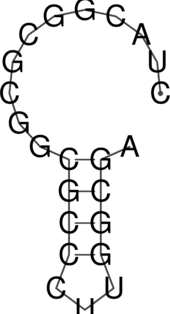
\includegraphics{Figs/test_ss.png}
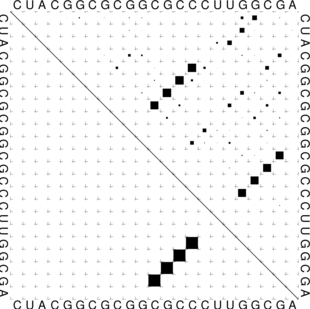
\includegraphics{Figs/test_dp.png}\\
The ``dot plot'' in \texttt{test\_dp.eps} shows the pair probabilities
within the equilibrium ensemble as \(n \times n\) matrix, and is an
excellent way to visualize structural alternatives. A square at row
\(i\) and column \(j\) indicates a base pair. The area of a square in
the upper right half of the matrix is proportional to the probability of
the base pair \(\left( {i,j} \right)\) within the equilibrium ensemble.
The lower left half shows all pairs belonging to the \texttt{MFE}
structure. While the MFE consists of a single helix, several different
helices are visualized in the pair probabilities.\\
 Next, let's use the \texttt{relplot} utility to visualize which parts
of a predicted MFE are well-defined and thus more reliable. Also let's
use a real example for a change and produce yet another representation
of the predicted structure, the \emph{mountain plot}.

\textbf{SHAPE directed RNA folding}\\
In order to further improve the quality of secondary structure
predictions, mapping experiments like SHAPE (selective 2'-hydroxyl
acylation analyzed by primer extension) can be used to exerimentally
determine the pairing status for each nucleotide. In addition to
thermodynamic based secondary structure predictions, RNAfold supports
the incorporation of this additional experimental data as soft
constraints.

If you want to use SHAPE data to guide the folding process, please make
sure that your experimental data is present in a text file, where each
line stores three white space separated columns containing the position,
the abbreviation and the normalized SHAPE reactivity for a certain
nucleotide.

\hyperdef{}{verbatim-26}{\label{verbatim-26}}
\begin{verbatim}
    1 G 0.134
    2 C 0.044
    3 C 0.057
    4 G 0.114
    5 U 0.094
      ...
      ...
      ...
    71 C 0.035
    72 G 0.909
    73 C 0.224
    74 C 0.529
    75 A 1.475
\end{verbatim}

The second column, which holds the nucleotide abbreviation, is optional.
If it is present, the data will be used to perform a cross check against
the provided input sequence. Missing SHAPE reactivities for certain
positions can be indicated by omitting the reactivity column or the
whole line. Negative reactivities will be treated as missing. Once the
SHAPE file is ready, it can be used to constrain folding:

\begin{verbatim}
$ RNAfold --shape=rna.shape --shapeMethod=D < rna.seq
\end{verbatim}

\subsubsection{The Program \texttt{RNApvmin}}{The Program RNApvmin}\label{the-program-rnapvmin}

The program \texttt{RNApvmin} reads a RNA sequence from \emph{stdin} and
uses an iterative minimization process to calculate a perturbation
vector that minimizes the discripancies between predicted pairing
probabilites and observed pairing probabilities (deduced from given
shape reactivities). The experimental SHAPE data has to be present in
the file format described above. The application will write the
calculated vector of perturbation energies to \emph{stdout}, while the
progress of the minimization process is written to \emph{stderr}. The
resulting perturbation vector can be interpreted directly and gives
usefull insights into the discrepancies between thermodynamic prediction
and experimentally determined pairing status. In addition the
perturbation energies can be used to constrain folding with
\texttt{RNAfold}:

\begin{verbatim}
$ RNApvmin rna.shape < rna.seq >vector.csv
$ RNAfold --shape=vector.csv --shapeMethod=W < rna.seq
\end{verbatim}

The perturbation vector file uses the same file format as the SHAPE data
file. Instead of SHAPE reactivities the raw perturbation energies will be
storred in the last column. Since the energy model is only adjusted when
necessary, the calculated perturbation energies may be used for the
interpretation of the secondary structure prediction, since they
indicate which positions require major energy model adjustments in order
to yield a prediction result close to the experimental data. High
perturbation energies for just a few nucleotides may indicate the
occurrence of features, which are not explicitly handled by the energy
model, such as posttranscriptional modifications and intermolecular
interactions.

\subsection{RNA-RNA Interactions}{RNA-RNA Interactions}\label{rna-rna-interactions}

A common problem is the prediction of binding sites between two RNAs, as
in the case of miRNA-mRNA interactions. Following tools of the
\texttt{ViennaRNA\ Package} can be used to calculate base pairing
probabilities.

\subsubsection{The Program \texttt{RNAcofold}}{The Program RNAcofold}\label{the-program-rnacofold}

\texttt{RNAcofold} works much like \texttt{RNAfold} but uses two RNA
sequences as input which are then allowed to form a dimer structure. In
the input the two RNA sequences should be concatenated using the
`\texttt{\&}' character as separator. As in \texttt{RNAfold} the
\texttt{-p} option can be used to compute partition function and base
pairing probabilities.\\
Since dimer formation is concentration dependent, \texttt{RNAcofold} can
be used to compute equilibrium concentrations for all five monomer and
(homo/hetero)-dimer species, given input concentrations for the monomers
(see the \texttt{man} page for details).

\textbf{Two Sequences one Structure}\\
1. Prepare a sequence file (\texttt{t.seq}) for input that looks like
this

\begin{verbatim}
``` {.commands}
>t
GCGCUUCGCCGCGCGCC&GCGCUUCGCCGCGCGCA
```

</div>
\end{verbatim}

\begin{enumerate}
\def\labelenumi{\arabic{enumi}.}
\setcounter{enumi}{1}
\tightlist
\item
  Compute the \texttt{MFE} and the ensemble properties
\item
  Look at the generated PostScript files \texttt{t\_ss.ps} and
  \texttt{t\_dp.ps}
\end{enumerate}

\begin{verbatim}
$ RNAcofold -p < t.seq
>t
GCGCUUCGCCGCGCGCC&GCGCUUCGCCGCGCGCA
((((..((..((((...&))))..))..))))... (-17.70)
((((..{(,.((((,,.&))))..}),.)))),,. [-18.26]
frequency of mfe structure in ensemble 0.401754 , delta G binding= -3.95
\end{verbatim}

\textbf{Secondary Structure Plot and Dot Plot}\\
 
\includegraphics{Figs/t_ss.png}
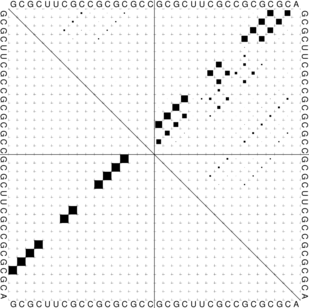
\includegraphics{Figs/t_dp.png}\\
In the dot plot a cross marks the chain break between the two
concatenated sequences.

\subsubsection{Concentration Dependency}{Concentration Dependency}\label{concentration-dependency}

Cofolding is an intermolecular process, therefore whether duplex
formation will actually occur is concentration dependent. Trivially, if
one of the molecules is not present, no dimers are going to be formed.
The partition functions of the molecules give us the equilibrium
constants:
-------------------------------------------------------------------------------------------------------------------------------------------
\[K_{AB} = \frac{\left\lbrack {AB} \right\rbrack}{\left\lbrack A \right\rbrack\left\lbrack B \right\rbrack} = \frac{Z_{AB}}{Z_{A}Z_{B}}\]
-------------------------------------------------------------------------------------------------------------------------------------------

with these and mass conservation, the equilibrium concentration of
homodimers, heterodimers and monomers can be computed in dependence of
the start concentrations of the two molecules. This is most easily done
by creating a file with the initial concentrations of molecules \(A\) and
\(B\) in two columns:\\
 \[\begin{array}{llll}
{\left\lbrack a_{1} \right\rbrack\left( \left\lbrack mol\slash l \right\rbrack \right)} & {\left\lbrack b_{1} \right\rbrack\left( \left\lbrack mol\slash l \right\rbrack \right)} & & \\
{\left\lbrack a_{2} \right\rbrack\left( \left\lbrack mol\slash l \right\rbrack \right)} & {\left\lbrack b_{2} \right\rbrack\left( \left\lbrack mol\slash l \right\rbrack \right)} & & \\
 \vdots & & & \\
{\left\lbrack a_{n} \right\rbrack\left( \left\lbrack mol\slash l \right\rbrack \right)} & {\left\lbrack b_{n} \right\rbrack\left( \left\lbrack mol\slash l \right\rbrack \right)} & & \\
\end{array}\]

\textbf{Concentration Dependency}\\
1. Prepare a concentration file for input with this little perl script

\begin{verbatim}
``` {.commands}
$ perl -e '$c=1e-07; do {print "$c\t$c\n"; $c*=1.71;} while $c<0.2' > concfile
```

This script creates a file displaying values from 1e-07 to just below
0.2, with 1.71-fold steps in between. For convenience, concentration
of molecule A is the same as concentration of molecule B in
each row. This will facilitate visualization of the results.
\end{verbatim}

\begin{enumerate}
\def\labelenumi{\arabic{enumi}.}
\setcounter{enumi}{1}
\tightlist
\item
  Compute the \texttt{MFE}, the ensemble properties and the
  concentration dependency of hybridization.

\begin{verbatim}
$ RNAcofold -f concfile < t.seq > cofold.out
\end{verbatim}
\item
  Look at the generated output with
\begin{verbatim}
$ less cofold.out
\end{verbatim}
\end{enumerate}

\begin{verbatim}
[...]
Free Energies:
AB              AA              BB              A               B
-18.261023      -17.562553      -18.274376      -7.017902       -7.290237
Initial concentrations          relative Equilibrium concentrations
A                B               AB              AA              BB              A               B
1e-07           1e-07           0.00003         0.00002         0.00002         0.49994         0.49993
[...]
\end{verbatim}

The five different free energies were printed out first, followed by a list
of all the equilibrium concentrations, where the first two columns denote
the initial (absolute) concentrations of molecules \(A\) and \(B\),
respectively. The next five columns denote the equilibrium concentrations
of dimers and monomers, relative to the total particle number. (Hence,
the concentrations don't add up to one, except in the case where no
dimers are built -- if you want to know the fraction of particles in a
dimer, you have to take the relative dimer concentrations times 2).\\
Since relative concentrations of species depend on two independent
values - initial concentration of A as well as initial concentration of
B - it is not trivial to visualize the results. For this reason we used
the same concentration for A and for B. Another possibility would be to
keep the initial concentration of one molecule constant. As an example
we show the following plot of \(t.seq\). Now we use some commandline
tools to render our plot. We use \texttt{tail\ -n\ +11} to show all
lines starting with line 11 (1-10 are cut) and pipe it into an
\texttt{awk} command, which prints every column but the first from our
input. This is then piped to \texttt{xmgrace}. With
\texttt{-log\ x\ -nxy\ -} we tell it to plot the x axis in logarithmic
scale and to read data file in X Y1 Y2 \ldots{} format.

\begin{verbatim}
$ tail -n +11 cofold.out | awk '{print $2, $3, $4, $5, $6, $7}' | xmgrace -log x -nxy -
\end{verbatim}

\textbf{Concentration Dependency plot}\\

\begin{center}\rule{0.5\linewidth}{\linethickness}\end{center}

\begin{figure}[htbp]
\centering
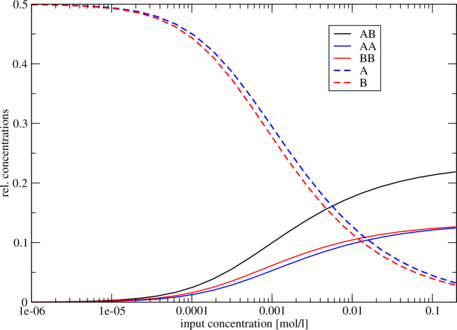
\includegraphics{Figs/tconcdep.png}
\caption{pict}
\end{figure}

\begin{center}\rule{0.5\linewidth}{\linethickness}\end{center}

\(\Delta G_{\text{binding}} = - 5.01\) kcal/mol

\begin{verbatim}
  sequences:GCGCUUCGCCGCGCGCG&GCGCUUCGCCGCGCGCG
\end{verbatim}

Since the two sequences are almost identical, the monomer and homo-dimer
concentrations behave very similarly. In this example, at a
concentration of about 1 mmol 50\% of the molecule is still in monomer
form.

\subsubsection{Finding potential binding sites with RNAduplex}{Finding potential binding sites with RNAduplex}\label{finding-potential-binding-sites-with-rnaduplex}

If the sequences are very long (many kb)\texttt{RNAcofold} is too slow
to be useful. The \texttt{RNAduplex} program is a fast alternative, that
works by predicting \emph{only} intermolecular base pairs. It's almost
as fast as simple sequence alignment, but much more accurate than a
\texttt{BLAST} search.

The example below searches the 3' UTR of an mRNA for a miRNA binding
site.

\textbf{Binding site prediction with RNAduplex}\\
 The file \texttt{duplex.seq} contains the 3'UTR of NM\_024615 and the
microRNA mir-145.

\begin{verbatim}
$ RNAduplex < duplex.seq
>NM_024615
>hsa-miR-145
.(((((.(((...((((((((((.&)))))))))))))))))).  34,57  :   1,19  (-21.90)
\end{verbatim}

Most favorable binding has an interaction energy of -21.90 kcal/mol and
pairs up on positions 34-57 of the UTR with positions 1-22 of the
miRNA.\\
 \texttt{RNAduplex} can also produce alternative binding sites,
e.g.~running \texttt{RNAduplex\ -e\ 10} would list all binding sites
within 10 kcal/mol of the best one.

Since \texttt{RNAduplex} forms only intermolecular pairs, it neglects
the competition between intramolecular folding and hybridization. Thus,
it is recommended to use \texttt{RNAduplex} as a pre-filter and analyse
good \texttt{RNAduplex} hits additionally with \texttt{RNAcofold} or
\texttt{RNAup}. Using the example above, running \texttt{RNAup} will
yield:

\begin{verbatim}
$ RNAup -b < duplex.seq

>NM_024615
>hsa-miR-145
(((((((&)))))))  50,56  :   1,7   (-8.41 = -9.50 + 0.69 + 0.40)
GCUGGAU&GUCCAGU
RNAup output in file: hsa-miR-145_NM_024615_w25_u1.out
\end{verbatim}

The free energy of the duplex is -9.50 kcal/mol and shows a discrepancy
to the structure and energy value computed by \texttt{RNAduplex}
(differences may arise from the fact that RNAup computes partition
functions rather than optimal structures). However, the total free
energy of binding is less favorable (-8.41 kcal/mol), since it includes
the energetic penalty for opening the binding site on the mRNA (0.69
kcal/mol) and miRNA (0.40 kcal/mol). The \texttt{-b} option includes the
probability of unpaired regions in both RNAs.

You can also run \texttt{RNAcofold} on the example to see the complete
structure after hybridization (neither \texttt{RNAduplex} nor
\texttt{RNAup} produce structure drawings). Note however, that the input
format for \texttt{RNAcofold} is different. An input file suitable for
\texttt{RNAcofold} has to be created from the \texttt{duplex.seq} file
first (use any text editor).\\
 As a more difficult example, let's look at the interaction of the
bacterial smallRNA RybB and its target mRNA ompN. First we'll try
predicting the binding site using RNAduplex:

\begin{verbatim}
$ RNAduplex < RybB.seq
>RybB
>ompN
.((((..((((((.(((....((((((((..(((((.((..((.((....((((..(((((((((((..((((((&
.))))))..))))))).)))).....))))....)).)).)).))).))..))))........))))..))).)))))).)))).
 5,79  :  80,164 (-34.60)
\end{verbatim}

Note, that the predicted structure spans almost the full length of the
RybB small RNA. Compare the predicted interaction to the structures
predicted for RybB and ompN alone, and ask yourself whether the
predicted interaction is indeed plausible.

Below the structure of ompN on the left and RybB on the right side. The
respective binding regions predicted by RNAduplex are marked in red.

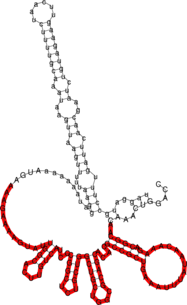
\includegraphics{Figs/ompN_ss.png}

\includegraphics{Figs/RybB_ss.png}

\begin{verbatim}
GCCAC-----TGCTTTTCTTTGATGTCCCCATTTT-GTGGA-------GC-CCATCAACCCCGCCATTTCGGTT---CAAG-GTTGGTGGGTTTTTT
 |||      ||||  |||||| |||    ||||| ||||        || ||| || ||  ||    ||||     |||| ||  |||  |||||| -40.30
AGGTCAAACAACGGC-AGAAACAATATT--TAAAGTCGCCGCACACGACGCGGTCGTCGGT-CGTCTCGGCCCTACTGTTCACGGTTATGAAAAGAAACC-3'
\end{verbatim}

Compare the \texttt{RNAduplex} prediction with the interaction predicted
by \texttt{RNAcofold}, \texttt{RNAup} and the handcrafted prediction you
see above.

\begin{figure}[htbp]
\centering
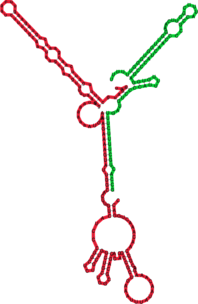
\includegraphics{Figs/OmpN_cofold.png}
\caption{pict}
\end{figure}

\subsection{Consensus Structure Prediction}{Consensus Structure Prediction}\label{consensus-structure-prediction}

Sequence co-variations are a direct consequence of RNA base pairing
rules and can be deduced to alignments. RNA helices normally contain
only 6 out of the 16 possible combinations: the Watson-Crick pairs GC,
CG, AU, UA, and the somewhat weaker wobble pairs GU and UG. Mutations in
helical regions therefore have to be correlated. In particular we often
find ``compensatory mutations'' where a mutation on one side of the helix
is compensated by a second mutation on the other side, e.g.~a
C\(\cdot\)G pair changes into a U\(\cdot\)A pair. Mutations where only
one pairing partner changes (such as C\(\cdot\)G to U\(\cdot\)G) are
termed ``consistent mutations''.

\subsubsection{The Program \texttt{RNAalifold}}{The Program RNAalifold}\label{the-program-rnaalifold}

\texttt{RNAalifold} generalizes the folding algorithm for sequence
alignments, treating the entire alignment as a single ``generalized
sequence''. To assign an energy to a structure on such a generalized
sequence, the energy is simply averaged over all sequences in the
alignment. This average energy is augmented by a covariance term, that
assigns a bonus or penalty to every possible base pair
\(\left( {i,j} \right)\) based on the sequence variation in columns
\(i\) and \(j\) of the alignment.\\
Compensatory mutations are a strong indication of structural
conservation, while consistent mutations provide a weaker signal. The
covariance term used by \texttt{RNAalifold} therefore assigns a bonus of
1 kcal/mol to each consistent and 2 kcal/mol for each compensatory
mutation. Sequences that cannot form a standard base pair incur a
penalty of \(- 1\) kcal/mol. Thus, for every possible consensus pair
between two columns \(i\) and \(j\) of the alignment a covariance score
\(C_{ij}\) is computed by counting the fraction of sequence pairs
exhibiting consistent and compensatory mutations, as well as the
fraction of sequences that are inconsistent with the pair. The weight of
the covariance term relative to the normal energy function, as well as
the penalty for inconsistent mutations can be changed via command line
parameters.\\
 Apart from the covariance term, the folding algorithm in
\texttt{RNAalifold} is essentially the same as for single sequence
folding. In particular, folding an alignment containing just one
sequence will give the same result as single sequence folding using
\texttt{RNAfold}. For \(N\) sequences of length \(n\) the required CPU
time scales as
\(\mathcal{\mathcal{O}}\left( {N \cdot n^{2} + n^{3}} \right)\) while
memory requirements grow as the square of the sequence length. Thus
\texttt{RNAalifold} is in general faster than folding each sequence
individually. The main advantage, however, is that the accuracy of
consensus structure predictions is generally much higher than for single
sequence folding, where typically only between 40\% and 70\% of the base
pairs are predicted correctly.\\
 Apart from prediction of \texttt{MFE} structures \texttt{RNAalifold}
also implements an algorithm to compute the partition function over all
possible (consensus) structures and the thermodynamic equilibrium
probability for each possible pair. These base pairing probabilities are
useful to see structural alternatives, and to distinguish well defined
regions, where the predicted structure is most likely correct, from
ambiguous regions.\\
 As a first example we'll produce a consensus structure prediction for
the following four tRNA sequences.

\begin{verbatim}
$ cat four.seq
\end{verbatim}

\begin{verbatim}
>M10740 Yeast-PHE
GCGGAUUUAGCUCAGUUGGGAGAGCGCCAGACUGAAGAUUUGGAGGUCCUGUGUUCGAUCCACAGAAUUCGCA
>K00349 Drosophila-PHE
GCCGAAAUAGCUCAGUUGGGAGAGCGUUAGACUGAAGAUCUAAAGGUCCCCGGUUCAAUCCCGGGUUUCGGCA
>K00283 Halobacterium volcanii Lys-tRNA-1
GGGCCGGUAGCUCAUUUAGGCAGAGCGUCUGACUCUUAAUCAGACGGUCGCGUGUUCGAAUCGCGUCCGGCCCA
>AF346993
CAGAGUGUAGCUUAACACAAAGCACCCAACUUACACUUAGGAGAUUUCAACUUAACUUGACCGCUCUGA
\end{verbatim}

\texttt{RNAalifold} uses aligned sequences as input. Thus, our first step
will be to align the sequences. We use \texttt{clustalw2} in this
example, since it's one of the most widely used alignment programs and
has been shown to work well on structural RNAs. Other alignment programs
can be used (including programs that attempt to do structural alignment
of RNAs), but the resulting multiple sequence alignment must be in
\texttt{Clustal} format. Get \texttt{clustalw2} and install it as you
have done it with the other packages:
\url{http://www.clustal.org/clustal2}

\textbf{Consensus Structure from related Sequences}\\
1. Prepare a sequence file (use file \texttt{four.seq} and copy it to your
working directory) 2. Align the sequences 3. Compute the consensus
structure from the alignment 4. Inspect the output files
\texttt{alifold.out}, \texttt{alirna.ps}, \texttt{alidot.ps} 5. For
comparison fold the sequences individually using \texttt{RNAfold}

\begin{verbatim}
$ clustalw2 four.seq > four.out
\end{verbatim}

\texttt{Clustalw2} creates two more output files, \texttt{four.aln} and
\texttt{four.dnd}. For \texttt{RNAalifold} you need the\texttt{.aln}
file.

\begin{verbatim}
$ RNAalifold -p four.aln
$ RNAfold -p < four.seq
\end{verbatim}

\texttt{RNAalifold} output:

\begin{verbatim}
__GCCGAUGUAGCUCAGUUGGG_AGAGCGCCAGACUGAAAAUCAGAAGGUCCCGUGUUCAAUCCACGGAUCCGGCA__
..(((((((..((((.........)))).(((((.......))))).....(((((.......))))))))))))...
 minimum free energy = -15.12 kcal/mol (-13.70 +  -1.43)
..(((((({..((((.........)))).(((((.......))))).....(((((.......)))))}))))))...
 free energy of ensemble = -15.75 kcal/mol
 frequency of mfe structure in ensemble 0.361603
..(((((((..((((.........)))).(((((.......))))).....(((((.......))))))))))))... -15.20 {-13.70 +  -1.50}
\end{verbatim}

\texttt{RNAfold} output:

\begin{verbatim}
>M10740 Yeast-PHE
GCGGAUUUAGCUCAGUUGGGAGAGCGCCAGACUGAAGAUUUGGAGGUCCUGUGUUCGAUCCACAGAAUUCGCA
((((((((........((((.((((((..((((...........))))..))))))..))))..)))))))). (-21.60)
((((((({...,,.{,((((.((((((..((((...........))))..))))))..))))),)))))))). [-23.20]
((((((((.........(((.((((((..((((...........))))..))))))..)))...)))))))). {-20.00 d=9.63}
 frequency of mfe structure in ensemble 0.0744065; ensemble diversity 15.35
>K00349 Drosophila-PHE
[...]
\end{verbatim}

The output contains a consensus sequence and the consensus structure in
dot-bracket notation. The consensus structure has an energy of
\(- 15.12\)~kcal/mol, which in turn consists of the average free energy
of the structure \(- 13.70\)~kcal/mol and the covariance term
\(- 1.43\)~kcal/mol. The strongly negative covariance term shows that
there must be a fair number of consistent and compensatory mutations,
but in contrast to the average free energy it's not meaningful in the
biophysical sense.

Compare the predicted consensus structure with the structures predicted
for the individual sequences using \texttt{RNAfold}. How often is the
correct ``clover-leaf'' shape predicted?

For better visualization, a structure annotated alignment or color
annotated structure drawing can be generated by using the
\texttt{-\/-aln} and \texttt{-\/-color} options of \texttt{RNAalifold}.

\begin{verbatim}
$ RNAalifold --color --aln four.aln
$ gv aln.ps &
$ gv alirna.ps &
\end{verbatim}

\textbf{\texttt{RNAalifold} Output Files}\\

\begin{verbatim}
4 sequence; length of alignment 78
alifold output
   6    72  0  99.8%   0.007 GC:2    GU:1    AU:1
  33    43  0  98.9%   0.033 GC:2    GU:1    AU:1
  31    45  0  99.0%   0.030 CG:3    UA:1
  15    25  0  98.9%   0.045 CG:3    UA:1
   5    73  1  99.7%   0.008 CG:2    GC:1
  13    27  0  99.1%   0.042 CG:4
  14    26  0  99.1%   0.042 UA:4
   4    74  1  99.5%   0.015 CG:3
[...]
\end{verbatim}

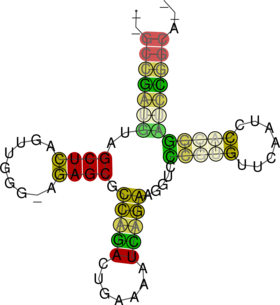
\includegraphics{Figs/alirna.png}
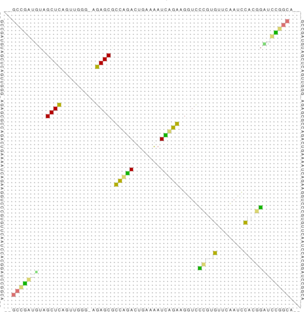
\includegraphics{Figs/alidot.png}

The last output file produced by \texttt{RNAalifold\ -p}, named
\texttt{alifold.out}, is a plain text file with detailed information on
all plausible base pairs sorted by the likelihood of the pair. In the
example above we see that the pair \(\left( {6,72} \right)\) has no
inconsistent sequences, is predicted almost with probability 1, and
occurs as a GC pair in two sequences, a GU pair in one, and a AU pair in
another.

\texttt{RNAalifold} automatically produces a drawing of the consensus
structure in Postscript format and writes it to the file
``\texttt{alirna.ps}''. In the structure graph consistent and
compensatory mutations are marked by a circle around the variable
base(s), i.e.~pairs where one pairing partner is encircled exhibit
consistent mutations, whereas pairs supported by compensatory mutations
have both bases marked. Pairs that cannot be formed by some of the
sequences are shown gray instead of black. In the example given, many
pairs show such inconsistencies. This is because one of the sequences
(AF346993) is not aligned well by \texttt{clustalw}.

Note, that subsequent calls to \texttt{RNAalifold} will overwrite any
existing output \texttt{alirna.ps} (\texttt{alidot.ps},
\texttt{alifold.out}) files in the current directory. Be sure to rename
any files you want to keep.

\textbf{Structure predictions for the individual sequences}\\
The consensus structure computed by \texttt{RNAalifold} will contain
only pairs that can be formed by most of the sequences. The structures
of the individual sequences will typically have additional base pairs
that are not part of the consensus structure. Moreover, ncRNA may
exhibit a highly conserved core structure while other regions are more
variable. It may therefore be desirable to produce structure predictions
for one particular sequence, while still using covariance information
from other sequences.

This can be accomplished by first computing the consensus structure for
all sequences using \texttt{RNAalifold}, then folding individual
sequences using \texttt{RNAfold\ -C} with the consensus structure as a
constraint. In constraint folding mode \texttt{RNAfold\ -C} allows only
base pairs to form which are compatible with the constraint structure.
This resulting structure typically contains most of the constraint (the
consensus structure) plus some additional pairs that are specific for
this sequence.

\subsubsection{RNAz}{RNAz}\label{rnaz}

\hyperdef{}{textcolor1}{\label{textcolor1}}{* New version by Someone who
loves RNAz. This part of the tutorial is based on the RNAz 1.0 version
which is obsolete quite a while already!!! *}\\
\texttt{AlifoldZ} has some shortcomings that limits its usefulness in
practice: The \(z\)-scores are not deterministic, i.e.~you get a
different score each time you run \texttt{AlifoldZ}. To get stable
\(z\)-scores you need to sample a large number of random alignments
which is computationally expensive. Moreover, \texttt{AlifoldZ} is
extremely sensitive to alignment errors.

The program \texttt{RNAz} overcomes these problems by using a different
approach to asses a multiple sequence alignment for significant RNA
structures. It is based on two key innovations: (i) The structure
conservation index (SCI) to measure structural conservation in an
alignment and (ii) \(z\)-scores that are calculated by regression
without sampling. Both measures are combined to an overall score that is
used to classify an alignment as ``structured RNA'' or ``other''.

\textbf{The structure conservation index}\\

\begin{figure}[htbp]
\centering
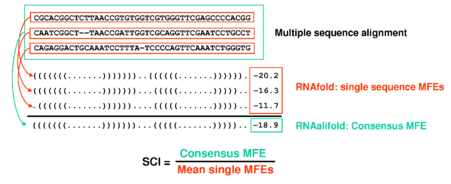
\includegraphics{Figs/sci.png}
\caption{pict}
\end{figure}

\begin{itemize}
\tightlist
\item
  The structure conservation index is an easy way to normalize an
  \texttt{RNAalifold} consensus MFE.
\end{itemize}

\textbf{z-score regression}\\
- The mean \(\mu\) and standard deviation \(\sigma\) of random samples
of a given sequence are functions of the length and the base
composition:
\[\mu,\sigma\left( {length,\frac{GC}{AT},\frac{G}{C},\frac{A}{T}} \right)\]
- It is therefore be possible to \emph{calculate} \(z\)-scores by
solving this 5 dimensional regression problem.

\textbf{SVM Classification}\\

\begin{figure}[htbp]
\centering
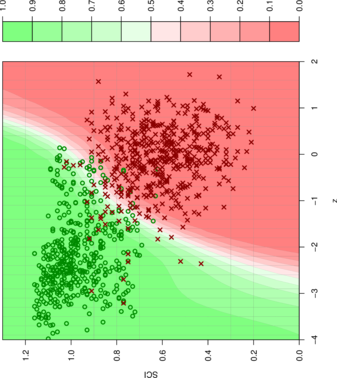
\includegraphics{Figs/contour.png}
\caption{pict}
\end{figure}

\begin{itemize}
\tightlist
\item
  A support vector machine learning algorithm is used to classify an
  alignment based on \(z\)-score and structure conservation index.
\end{itemize}

\textbf{Basic usage of RNAz}\\
 \hyperdef{}{textcolor2}{\label{textcolor2}}{* where to get examples
from (RNAz install package) - commands work with v2 but txt needs to be
adopted *} - \texttt{RNAz} reads one or more multiple sequence
alignments in \texttt{clustalw} or MAF format.

\begin{verbatim}
$ RNAz --help
$ RNAz tRNA.aln
$ RNAz --both-strands --predict-strand tRNA.maf
\end{verbatim}

\textbf{Advanced usage of RNAz}\\
- \texttt{RNAz} is limited to a maximum alignment length of 400 columns
and a maximum number of 6 sequences. To process larger alignments a set
of Perl helper scripts are used. - Selecting one or more subsets of
sequences from an alignment with more than 6 sequences:

\begin{verbatim}
$ rnazSelectSeqs.pl miRNA.maf |RNAz
$ rnazSelectSeqs.pl --num-seqs=4 --num-samples=3 miRNA.maf |RNAz
\end{verbatim}

\begin{itemize}
\tightlist
\item
  Scoring long alignments in overlapping windows:
\end{itemize}

\begin{verbatim}
$ rnazWindow.pl --window=120 --slide=40 unknown.aln \
              | RNAz --both-strands
\end{verbatim}

\subsubsection{Large scale screens}{Large scale screens}\label{large-scale-screens}

The \texttt{RNAz} package provides a set of Perl scripts that implement
a complete analysis pipeline suitable for medium to large scale screens
of genomic data.

\textbf{General procedure}\\
1. Obtain or create multiple sequence alignments in MAF format 2. Run
through the \texttt{RNAz} pipeline:

\begin{figure}[htbp]
\centering
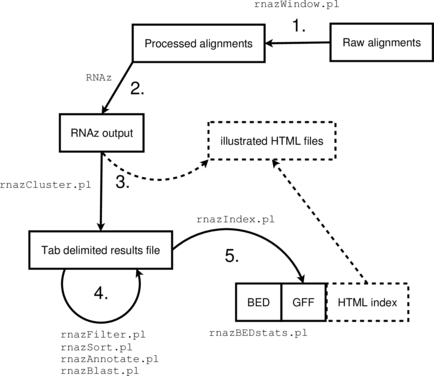
\includegraphics{Figs/flowchart.png}
\caption{pict}
\end{figure}

\textbf{Examples in this tutorial}\\
1. Align Epstein Barr Virus genome (Acc.no: NC\_007605) to two related
primate viruses (Acc.nos: NC\_004367, NC\_006146) using \texttt{multiz}
and run it through the \texttt{RNAz} pipeline.
\hyperdef{}{textcolor3}{\label{textcolor3}}{* where are this data
comeing from? file from NCBI differs from those hidden in
genefinding/rnaz/herpes *} 2. Analyze snoRNA cluster in the human genome
for conserved RNA structures: download pre-computed alignments from the
UCSC genome browser and run it through the \texttt{RNAz} pipeline

\textbf{Example a: Preparation of data}\\
- \texttt{multiz} and \texttt{blastz} are available here:
\url{http://www.bx.psu.edu/miller_lab/} - Download the viral genomes in
FASTA format and reformat the header strictly according to the rules
given in the \texttt{multiz} documentation
(\url{http://www.bx.psu.edu/miller_lab/dist/tba_howto.pdf}), e.g.: - You
have to edit the ''multiz '' \texttt{Makefile} and replace

\begin{verbatim}
<div id="verbatim-88" class="verbatim">

``` {.commands}
CFLAGS = -Wall -Wextra -Werror
```

</div>

with

<div id="verbatim-89" class="verbatim">

``` {.commands}
CFLAGS = -Wall -Wextra #-Werror
```

</div>

and then simply use the `make` command to compile both programs.
\end{verbatim}

\hyperdef{}{textcolor4}{\label{textcolor4}}{* dont understand what to do
*}

\hyperdef{}{verbatim-90}{\label{verbatim-90}}
\begin{verbatim}
>NC_007605:genome:1:+:149696
AGAATTCGTCTTGCTCTATTCACCCTTACTTTTCTTCTTGCCCGTTCTCTTTCTTAGTAT
GAATCCAGTATGCCTGCCTGTAATTGTTGCGCCCTACCTCTTTTGGCTGGCGGCTATTGC
CGCCTCGTGTTTCACGGCCTCAGTTAGTACCGTTGTGACCGCCACCGGCTTGGCCCTCTC
ACTTCTACTCTTGGCAGCAGTGGCCAGCTCATATGCCGCTGCACAAAGGAAACTGCTGAC
ACCGGTGACAGTGCTTACTGCGGTTGTCACTTGTGAGTACACACGCACCATTTACAATGC
ATGATGTTCGTGAGATTGATCTGTCTCTAACAGTTCACTTCCTCTGCTTTTCTCCTCAGT
CTTTGCAATTTGCCTAACATGGAGGATTGAGGACCCACCTTTTAATTCTCTTCTGTTTGC
[...]
\end{verbatim}

\textbf{Example a: Aligning viral genomes}\\
- To get a multiple alignment a phylogenetic tree and the following
three steps are necessary: 1. Run \texttt{blastz} each vs.~each 2.
Combine blastz results to multiple sequence alignments 3. Project raw
alignments to a reference sequence. - The corresponding commands:

\begin{verbatim}
all_bz - "((NC_007605 NC_006146) NC_004367)" | bash
tba "((NC_007605 NC_006146) NC_004367)" \
*.sing.maf raw-tba.maf
maf_project raw-tba.maf NC_007605 > final.maf
\end{verbatim}

\begin{itemize}
\tightlist
\item
  Note: The tree is given in NEWICK like format with blanks instead of
  commas. The sequence data files must be named exactly like the names in
  this tree and in the FASTA headers.
\end{itemize}

\textbf{Example a: Running the pipeline I}\\
- First the alignments are filtered and sliced in overlapping windows:

\begin{verbatim}
$ rnazWindow.pl < final.maf > windows.maf
\end{verbatim}

\begin{itemize}
\tightlist
\item
  \texttt{RNAz} is run on these windows:
\end{itemize}

\begin{verbatim}
$ RNAz --both-strands --show-gaps --cutoff=0.5 windows.maf \
       > rnaz.out
\end{verbatim}

\begin{itemize}
\tightlist
\item
  Overlapping hits are combined to ``loci'' and visualized on a
  web-site:
\end{itemize}

\begin{verbatim}
$ rnazCluster.pl --html rnaz.out > results.dat
\end{verbatim}

\textbf{Example a: Running the pipeline II}\\
- The predicted hits are compared with available annotation of the
genome:

\begin{verbatim}
$ rnazAnnotate.pl --bed annotation.bed results.dat \
         > results_annotated.dat
\end{verbatim}

\begin{itemize}
\tightlist
\item
  The results file is formatted in a HTML overview page:
\end{itemize}

\begin{verbatim}
$ rnazIndex.pl --html results_annotated.dat \
         > results/index.html
\end{verbatim}

\textbf{Example a: Statistics on the results}\\
- \texttt{rnazIndex.pl} can be used to generate a BED formatted
annotation file which can be analyzed using \texttt{rnazBEDstats.pl}
(after sorting, for the case the input alignments were unsorted)''

\begin{verbatim}
$ rnazIndex.pl --bed results.dat | \
         rnazBEDsort.pl | rnazBEDstats.pl
\end{verbatim}

\begin{itemize}
\tightlist
\item
  RNAzfilter.pl can be used to filter the results by different criteria. In
  this case it gives us all loci with P\$\textgreater{}\$0.9'':
\end{itemize}

\begin{verbatim}
$ rnazFilter.pl "P>0.9" results.dat | \
         rnazIndex.pl --bed | \
         rnazBEDsort.pl | rnazBEDstats.pl
\end{verbatim}

\begin{itemize}
\tightlist
\item
  To get an estimate on the (statistical) false positives one can repeat
  the complete screen with randomized alignments:
\end{itemize}

\begin{verbatim}
$ rnazRandomizeAln final.maf > random.maf
\end{verbatim}

\textbf{Example b: Obtaining pre-computed alignments from UCSC}\\
- Go to the UCSC genome browser
(\href{http://genome.ucsc.edu/}{http://genome.ucsc.edu}) and go to
``Tables''. Download ``multiz17'' alignments in MAF format for the
region: chr11:93103000-93108000

\begin{figure}[htbp]
\centering
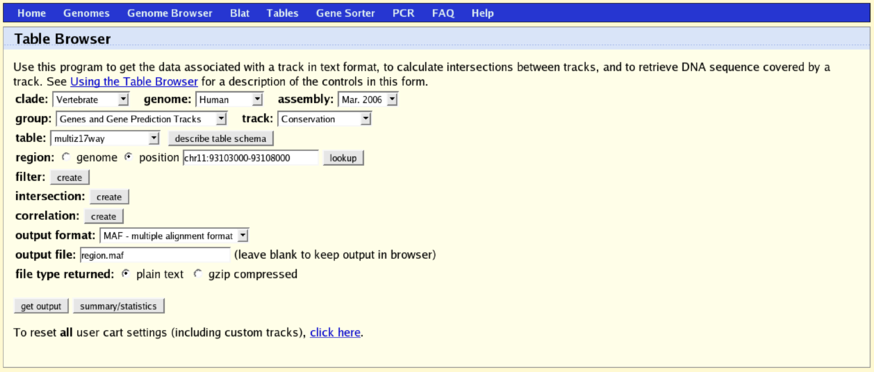
\includegraphics{Figs/table-browser.png}
\caption{pict}
\end{figure}

\textbf{Example b: Running the pipeline}\\
- The Perl scripts are run in the same order as in Example 1:

\begin{verbatim}
$ rnazWindow.pl --min-seqs=4 region.maf > windows.maf
$ RNAz --both-strands --show-gaps --cutoff=0.5 windows.maf \
         > rnaz.out
$ rnazCluster.pl --html rnaz.out > results.dat
$ rnazAnnotate.pl --bed annotation.bed results.dat \
         > results_annotated.dat
$ rnazIndex.pl --html results_annotated.dat \
         > results/index.html
\end{verbatim}

\begin{itemize}
\tightlist
\item
  The results can be exported as UCSC BED file which can be displayed in
  the genome browser:
\end{itemize}

\begin{verbatim}
$ rnazIndex.pl --bed --ucsc results.dat > prediction.bed
\end{verbatim}

\textbf{Example b: Visualizing the results on the genome browser}\\
- Upload the BED file as ``Custom Track''\ldots{}

\begin{figure}[htbp]
\centering
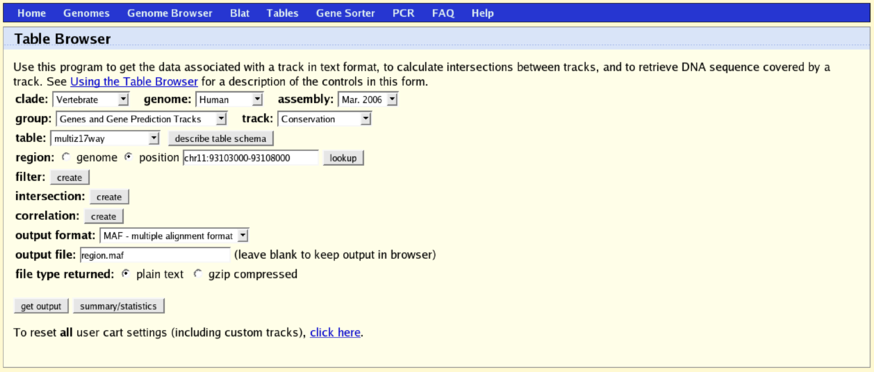
\includegraphics{Figs/table-browser.png}
\caption{pict}
\end{figure}

\begin{itemize}
\tightlist
\item
  \ldots{}and have a look at the results:
\end{itemize}

\begin{figure}[htbp]
\centering

\includegraphics{Figs/snos.png}
\caption{pict}
\end{figure}

\textbackslash{}let \textbackslash{}prOteCt \textbackslash{}relax
\textbackslash{}Protect \textbackslash{}gl:nopartrue

\hyperdef{}{sidebar}{\label{sidebar}}
\begin{itemize}
\tightlist
\item
  \hyperref[sec1]{RNA Web Services{}}

  \begin{itemize}
  \tightlist
  \item
    \hyperref[sec1]{Useful Web Services}
  \end{itemize}
\item
  \hyperref[sec2]{Get started{}}

  \begin{itemize}
  \tightlist
  \item
    \hyperref[sec2ux5f1]{Typographical Conventions}
  \item
    \hyperref[sec2ux5f2]{Data Files}
  \item
    \hyperref[sec2ux5f3]{Terminal, Command line and Editor}
  \item
    \hyperref[sec2ux5f4]{Installing Software from Source}
  \item
    \hyperref[sec2ux5f5]{Build the \texttt{ViennaRNA\ Package}}
  \item
    \hyperref[sec2ux5f6]{What's in the \texttt{ViennaRNA\ Package}}
  \item
    \hyperref[sec2ux5f7]{The Input File Format}
  \end{itemize}
\item
  \hyperref[sec3]{Structure Prediction on single Sequences{}}

  \begin{itemize}
  \tightlist
  \item
    \hyperref[sec3ux5f1]{The Program \texttt{RNAfold}}
  \item
    \hyperref[sec3ux5f2]{The Program \texttt{RNApvmin}}
  \item
    \hyperref[sec3ux5f3]{The Program \texttt{RNAsubopt}}
  \end{itemize}
\item
  \hyperref[sec4]{RNA folding kinetics{}}

  \begin{itemize}
  \tightlist
  \item
    \hyperref[sec4ux5f1]{RNA2Dfold}
  \item
    \hyperref[sec4ux5f2]{barriers \& treekin}
  \end{itemize}
\item
  \hyperref[sec5]{Sequence Design{}}

  \begin{itemize}
  \tightlist
  \item
    \hyperref[sec5ux5f1]{The Program \texttt{RNAinverse}}
  \item
    \hyperref[sec5ux5f2]{switch.pl}
  \end{itemize}
\item
  \hyperref[sec6]{RNA-RNA Interactions{}}

  \begin{itemize}
  \tightlist
  \item
    \hyperref[sec6ux5f1]{The Program \texttt{RNAcofold}}
  \item
    \hyperref[sec6ux5f2]{Concentration Dependency}
  \item
    \hyperref[sec6ux5f3]{Finding potential binding sites with RNAduplex}
  \end{itemize}
\item
  \hyperref[sec7]{Consensus Structure Prediction{}}

  \begin{itemize}
  \tightlist
  \item
    \hyperref[sec7ux5f1]{The Program \texttt{RNAalifold}}
  \end{itemize}
\item
  \hyperref[sec8]{Structural Alignments{}}

  \begin{itemize}
  \tightlist
  \item
    \hyperref[sec8ux5f1]{Manually correcting Alignments}
  \item
    \hyperref[sec8ux5f2]{Automatic structural alignments}
  \end{itemize}
\item
  \hyperref[sec9]{Noncoding RNA gene prediction{}}

  \begin{itemize}
  \tightlist
  \item
    \hyperref[sec9ux5f1]{QRNA}
  \item
    \hyperref[sec9ux5f2]{AlifoldZ}
  \item
    \hyperref[sec9ux5f3]{RNAz}
  \item
    \hyperref[sec9ux5f4]{Large scale screens}
  \end{itemize}
\end{itemize}

\hyperref[]{Top}

\href{https://www.tbi.univie.ac.at/legal.html}{Legal Details}

\end{document}
